\genHeader \fancyfoot[ER]{  $\triangleright$ \hyperlink{installPlugin common}{Next} } {\small \texttt Approximate time: Just a few minutes \ldots}

This part provides a very simple example and a JUnit test to check the installation and configuration of eMoflon.

After working through this part, you should have an installed and tested eMoflon working for a trivial example. We also explain the general workflow, the
different workspaces involved and general useage of each syntax.

This part can be considered \emph{mandatory} if you are new to eMoflon, but we reccommend working through it anyway.

Here's how we've organized our handbooks; in this part we introduce the first black, red, and blue headers to separate the common, visual, and textual syntax
instructions (Fig~\ref{pageExamples}).

\begin{figure}[htbp] \centering
  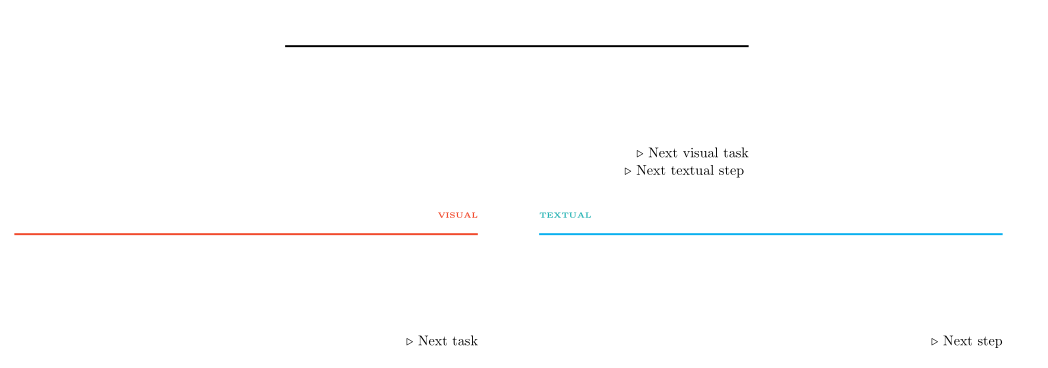
\includegraphics[width=1\textwidth]{pageExamples}
	\caption{Page Headers and Links} 
	\label{pageExamples} 
\end{figure}

At the end of each section, you'll find a \mbox{ $\triangleright$ {\texttt Next {\emph{label}}} } link. This is the link that will take you to the next
appropriate page. You are still welcome to go through the entire handbook page by page. In fact, we encourage it for our diagrams! We hope you can compare the
differences and similarities between the two sytanxes. But be warned - If what you're doing isn't matching what you see, you may be reading the wrong
instructions.

\pagebreak

If, however, you're finding that the screenshots we've taken aren't matching your screen and you ARE in the right place, please send us an email at
\href{mailto:contact@moflon.org}{contact@moflon.org} and let us know. They get outdated so fast! They just grow up, move on, start doing their own thing and
\ldots uh, wait a second. We're talking about pictures here.

Feel free to also contact us if you have any questions, concerns, or suggestions on ways we can improve.

\newpage